\documentclass[12pt,a4paper]{article}
%% ntts2019abstract..tex - https://ec.europa.eu/eurostat/cros/system/files/ntts2019abstract_tex.zip
%% TEMPLATE FOR NTTS 2019 CONFERENCE
%% This LaTex source file is (coarsely) following the corresponding DOT template document of
%% the conference (https://ec.europa.eu/eurostat/cros/system/files/ntts2019abstract.dot)
%% Prepared by J.Grazzini (Eurostat, unit B1)

\def\thisfile{ntts2019abstract}

%% WHO ARE YOU: LIST THE AUTHORS HERE
\def\theauthors{
%Alain Quartier-la-Tente
}

%% WHAT IS YOUR PAPER ABOUT: PUT YOUR TITLE HERE
\def\thetitle{
\textbf{{RJDemetra: an R interface to JDemetra+}
}
}

%% TELL US MORE... THROUGH KEYWORDS!
\def\thekeywords{
\textit{Seasonal adjustment, R, JDemetra+}.
}

%% PLEASE KEEP AT LIST THESE SETTINGS
\def\thepaperheight{29.9cm} 	% original: {11.99in}
\def\thepaperwidth{21.08cm} 	% 		{8.3in}
\def\theleft{2.79cm} 			% 		{1.1in}
\def\theright{2.99cm} 			%		{1.18in}
\def\thetop{1.7cm} 			% 		{0.51in}
\def\thebottom{1.6cm} 		% 		{0.71in}
\def\theheadheight{2.54cm} 	% 		(1in}

\usepackage[
   a4paper,
   paperheight=\thepaperheight,
   paperwidth=\thepaperwidth,
   left=\theleft,
   right=\theright,
   top=\thetop,
   bottom=\thebottom,
   headheight=\theheadheight
]{geometry} % in particular, do not change the dimensions of the document



\usepackage{color}
\usepackage{fancyvrb}
\newcommand{\VerbBar}{|}
\newcommand{\VERB}{\Verb[commandchars=\\\{\}]}
\DefineVerbatimEnvironment{Highlighting}{Verbatim}{commandchars=\\\{\}}
% Add ',fontsize=\small' for more characters per line
\usepackage{framed}
\definecolor{shadecolor}{RGB}{248,248,248}
\newenvironment{Shaded}{\begin{snugshade}}{\end{snugshade}}
\newcommand{\KeywordTok}[1]{\textcolor[rgb]{0.13,0.29,0.53}{\textbf{#1}}}
\newcommand{\DataTypeTok}[1]{\textcolor[rgb]{0.13,0.29,0.53}{#1}}
\newcommand{\DecValTok}[1]{\textcolor[rgb]{0.00,0.00,0.81}{#1}}
\newcommand{\BaseNTok}[1]{\textcolor[rgb]{0.00,0.00,0.81}{#1}}
\newcommand{\FloatTok}[1]{\textcolor[rgb]{0.00,0.00,0.81}{#1}}
\newcommand{\ConstantTok}[1]{\textcolor[rgb]{0.00,0.00,0.00}{#1}}
\newcommand{\CharTok}[1]{\textcolor[rgb]{0.31,0.60,0.02}{#1}}
\newcommand{\SpecialCharTok}[1]{\textcolor[rgb]{0.00,0.00,0.00}{#1}}
\newcommand{\StringTok}[1]{\textcolor[rgb]{0.31,0.60,0.02}{#1}}
\newcommand{\VerbatimStringTok}[1]{\textcolor[rgb]{0.31,0.60,0.02}{#1}}
\newcommand{\SpecialStringTok}[1]{\textcolor[rgb]{0.31,0.60,0.02}{#1}}
\newcommand{\ImportTok}[1]{#1}
\newcommand{\CommentTok}[1]{\textcolor[rgb]{0.56,0.35,0.01}{\textit{#1}}}
\newcommand{\DocumentationTok}[1]{\textcolor[rgb]{0.56,0.35,0.01}{\textbf{\textit{#1}}}}
\newcommand{\AnnotationTok}[1]{\textcolor[rgb]{0.56,0.35,0.01}{\textbf{\textit{#1}}}}
\newcommand{\CommentVarTok}[1]{\textcolor[rgb]{0.56,0.35,0.01}{\textbf{\textit{#1}}}}
\newcommand{\OtherTok}[1]{\textcolor[rgb]{0.56,0.35,0.01}{#1}}
\newcommand{\FunctionTok}[1]{\textcolor[rgb]{0.00,0.00,0.00}{#1}}
\newcommand{\VariableTok}[1]{\textcolor[rgb]{0.00,0.00,0.00}{#1}}
\newcommand{\ControlFlowTok}[1]{\textcolor[rgb]{0.13,0.29,0.53}{\textbf{#1}}}
\newcommand{\OperatorTok}[1]{\textcolor[rgb]{0.81,0.36,0.00}{\textbf{#1}}}
\newcommand{\BuiltInTok}[1]{#1}
\newcommand{\ExtensionTok}[1]{#1}
\newcommand{\PreprocessorTok}[1]{\textcolor[rgb]{0.56,0.35,0.01}{\textit{#1}}}
\newcommand{\AttributeTok}[1]{\textcolor[rgb]{0.77,0.63,0.00}{#1}}
\newcommand{\RegionMarkerTok}[1]{#1}
\newcommand{\InformationTok}[1]{\textcolor[rgb]{0.56,0.35,0.01}{\textbf{\textit{#1}}}}
\newcommand{\WarningTok}[1]{\textcolor[rgb]{0.56,0.35,0.01}{\textbf{\textit{#1}}}}
\newcommand{\AlertTok}[1]{\textcolor[rgb]{0.94,0.16,0.16}{#1}}
\newcommand{\ErrorTok}[1]{\textcolor[rgb]{0.64,0.00,0.00}{\textbf{#1}}}
\newcommand{\NormalTok}[1]{#1}
\usepackage{grffile}

\usepackage{fancyhdr}

%\cfoot{ {\fontsize{8pt}{9.6pt}\selectfont 6\par}}

%% NO HEADING...
%%\fancyhead[RE]{\headreport}
%%\fancyhead[RO,LE]{\bfseries\thepage}
%%\fancyhead[LO]{\nouppercase{\rightmark}} %{\markright} %{\sectionmark}

\pagestyle{fancy}
\fancyhf{}

% you can use hyperref as set below once the colorboxes are gone...
\usepackage[pdfauthor={\theauthors}, pdftitle={\thetitle}]{hyperref}
% otherwise simply stick to that one
%\usepackage{hyperref}

\hypersetup{colorlinks=true,       % false: boxed links; true: colored links
    % linkcolor=blue,          % color of internal links
    citecolor=red,        % color of links to bibliography
    filecolor=magenta,      % color of file links
    urlcolor=cyan           % color of external links
}
%% or:
% \usepackage[hidelinks]{hyperref} % make links black

\usepackage{sectsty}
\usepackage{setspace}

\renewcommand{\headrulewidth}{0pt}
\setlength{\topsep}{0pt}\setlength{\parindent}{0pt}

\renewcommand{\arraystretch}{1.3}

%% depths for Sections 
% 1) Section
% 1.1) SubSection
% 1.1.1) SubSubSection
% 1.1.1.1) Paragraph
\setcounter{tocdepth}{4}
\setcounter{secnumdepth}{4}

% depths for nested lists created by \begin{enumerate}
\usepackage{enumitem}
\setlistdepth{9}
\renewlist{enumerate}{enumerate}{9}
	\setlist[enumerate,1]{label=\arabic*)}
	\setlist[enumerate,2]{label=\alph*)}
	\setlist[enumerate,3]{label=(\roman*)}
	\setlist[enumerate,4]{label=(\arabic*)}
	\setlist[enumerate,5]{label=(\Alph*)}
	\setlist[enumerate,6]{label=(\Roman*)}
	\setlist[enumerate,7]{label=\arabic*}
	\setlist[enumerate,8]{label=\alph*}
	\setlist[enumerate,9]{label=\roman*}
\renewlist{itemize}{itemize}{9}
	\setlist[itemize]{label=$\cdot$}
	\setlist[itemize,1]{label=\textbullet}
	\setlist[itemize,2]{label=$\circ$}
	\setlist[itemize,3]{label=$\ast$}
	\setlist[itemize,4]{label=$\dagger$}
	\setlist[itemize,5]{label=$\triangleright$}
	\setlist[itemize,6]{label=$\bigstar$}
	\setlist[itemize,7]{label=$\blacklozenge$}
	\setlist[itemize,8]{label=$\prime$}

% that's for generating directly PDF documents using pdfLaTex instead of LaTex alone
\newif\ifpdf\ifx\pdfoutput\undefined\pdffalse\else\pdfoutput=1\pdftrue\fi
\newcommand{\pdfgraphics}{\ifpdf\DeclareGraphicsExtensions{.pdf,.png,.tif,.jpg}\else\fi}

%% KEEP THIS FOR THE EXAMPLES BELOW TO RUN...OR RUN YOUR OWN
% \usepackage[boxed]{algorithm2e}
\usepackage{algorithm}
%\usepackage{algorithmic}
\usepackage[noend]{algpseudocode}
\makeatletter\def\BState{\State\hskip-\ALG@thistlm}\makeatother

%% DEAL WITH THE BIBLIOGRAPHY

% that's what we use here for the bibliography
\usepackage[numbers]{natbib}
% see https://gking.harvard.edu/files/natnotes2.pdf
\newcommand*{\doi}[1]{DOI: \href{https://doi.org/\detokenize{#1}}{\detokenize{#1}}} 
\newcommand*{\arxiv}[1]{arXiv: \href{https://arxiv.org/abs/\detokenize{#1}}{\detokenize{#1}}} 


%% If you are compiling using biblatex
%\usepackage[
%    backend=biber,
%    style=authoryear,
%    natbib=true,
%    url=true, 
%    doi=true,
%    eprint=false, 
%    sorting=ynt
%]{biblatex}
%\addbibresource{\thisfile.bib}


\usepackage[utf8]{inputenc}
\usepackage[T1]{fontenc}

\usepackage{amsmath}
\usepackage{latexsym}
\usepackage{amsfonts}
\usepackage[normalem]{ulem}
\usepackage{array}
\usepackage{amssymb}

\ifpdf
\usepackage[pdftex]{graphicx}
\else
\usepackage{graphicx}
\fi

%\graphicspath{
%
%}

\usepackage{float}
%\usepackage{subfloat}
\usepackage{subfig}
% \usepackage[list=true]{subcaption} % cannot be used conjointly with subfig
\usepackage{wrapfig}
\usepackage{wasysym}
\usepackage[svgnames,table]{xcolor}
\usepackage{longtable} % long tabulars
\usepackage{adjustbox}
\usepackage{alltt} % verbatim 
\usepackage{changepage}
\usepackage{hhline}
\usepackage{multicol}
\usepackage{tabto}
\usepackage{multirow}
%\usepackage{ragged2e}
%\usepackage{tikz}
%\usepackage{makecell}
%\usepackage[toc,page]{appendix}

\urlstyle{same}


 %% HEADER
\title{
\vspace{-5ex}
\thetitle
\vspace{-2ex}
}
\author{
\theauthors
\vspace{-5ex}
}
\date{}


%% YOUR DOCUMENT STARTS HERE

\begin{document}
\cfoot{\thepage} % keep pages numbered

%% PLEASE KEEP THIS FORMATTING
\sectionfont{\large\textsc}
%\sectionfont{\large\MakeUppercase}
%%

\maketitle

{\fontsize{10pt}{12.0pt}\selectfont \textbf{\uline{Keywords}:} \thekeywords\par}\par


\section{Introduction}\label{introduction}

RJDemetra is a R interface to
\href{https://github.com/jdemetra/jdemetra-app}{JDemetra+}, the seasonal
adjustment software
\href{https://ec.europa.eu/eurostat/cros/system/files/Jdemetra_\%20release.pdf}{officially
recommended} by Eurostat and the European Central Bank (ECB) to the members of the European Statistical System (ESS) and the European System of Central Banks (ESCB).

JDemetra+ is a developed by the National Bank of Belgium (NBB) in
cooperation with the Deutsche Bundesbank with the support of Eurostat, in accordance with
the ESS Guidelines on Seasonal Adjustment. It implements the two leading seasonal adjustment methods
\href{http://www.bde.es/bde/en/secciones/servicios/Profesionales/Programas_estadi/Programas_estad_d9fa7f3710fd821.html}{TRAMO/SEATS+} \cite{gomez1998automatic,caporello2004program}
and
\href{https://www.census.gov/srd/www/x13as/}{X-12ARIMA/X-13ARIMA-SEATS}~\cite{findleyx12,ladiray1999x11}.

R is a programming language and free software environment for
statistical computing and free software widely use by statisticians.

RJDemetra is a R package that offers full access to all JDemetra+ options and
outputs. It also offers many possibilities to the users to implement new tools for the production of seasonally
adjusted series thanks to all the libraries already available in R. RJDemetra is
available on github: \url{https://github.com/nbbrd/RJDemetra}.

\section{Methods}\label{methods}

RJDemetra relies on the Java libraries use in JDemetra+: the algorithms
are not implemented inside the package. The link between R and Java
libraries is done with the
\href{https://CRAN.R-project.org/package=rJava}{rJava} package, which is
a low-level R to Java interface. The consequence is that the results of
the seasonal adjustment done using R are certified by the use of JDemetra+
and the system requirements needed to install the package are the same
needed to use JDemetra+ (Java SE 8 or later).

The goal of the RJDemetra package is to offer a ``pure R'' package to
the users, more familiar with this language rather than with Java. It allows an easy integration of the seasonal adjustment process in IT production systems and offers the possibility to implements new tools that are difficult to integrate into the graphical interface of JDemetra+, as for examples:

\begin{itemize}
\item
  The comparison of the direct and indirect adjustments;
\item
  The automatic generation of dashboards to summarise the information on the seasonal adjustment ;
\item
  The generation of quality reports.
\end{itemize}

\section{Results}\label{results}

In the current version of the RJDemetra package, users can:

\begin{itemize}
\item
  Seasonally adjust their time series with the TRAMO-SEATS and/or X-13-ARIMA;
\item
  Use the regARIMA-based preadjustment method implemented in TRAMO-SEATS and X-13-ARIMA;
\item
  Manipulate JDemetra+ workspaces to easily switch to the JDemetra+ graphical interface. The current functionalities are:

  \begin{itemize}
  \item
    Import of JDemetra+ workspace in R (raw data and seasonal adjustment specifications);
  \item
    Export of specifications created via RJDemetra to a JDemetra+ workspace.
  \end{itemize}
\end{itemize}

All seasonally adjust objects created by RJDemetra are S3 classes \cite{wickham2014advanced} with basic methods: \texttt{print()}, \texttt{plot()} and
\texttt{summary()} (for regARIMA models).

Let's see an example with the French manufacturing industrial production index
(\url{https://www.insee.fr/en/statistiques/serie/010537903}). The time
series can be seasonally adjusted with the X-13-ARIMA method using the
function \texttt{x13\_def()}. The main results are presented in figure
\ref{fig:sa_ipi} created by the \texttt{plot()} function.

\begin{Shaded}
\begin{Highlighting}[]
\KeywordTok{library}\NormalTok{(RJDemetra)}
\NormalTok{x13_ipi <-}\StringTok{ }\KeywordTok{x13_def}\NormalTok{(ipi_french, }\DataTypeTok{spec =} \StringTok{"RSA3"}\NormalTok{)}
\KeywordTok{plot}\NormalTok{(x13_ipi, }\DataTypeTok{type_chart =} \StringTok{"sa-trend"}\NormalTok{)}
\end{Highlighting}
\end{Shaded}

\begin{figure}[H]
\centering
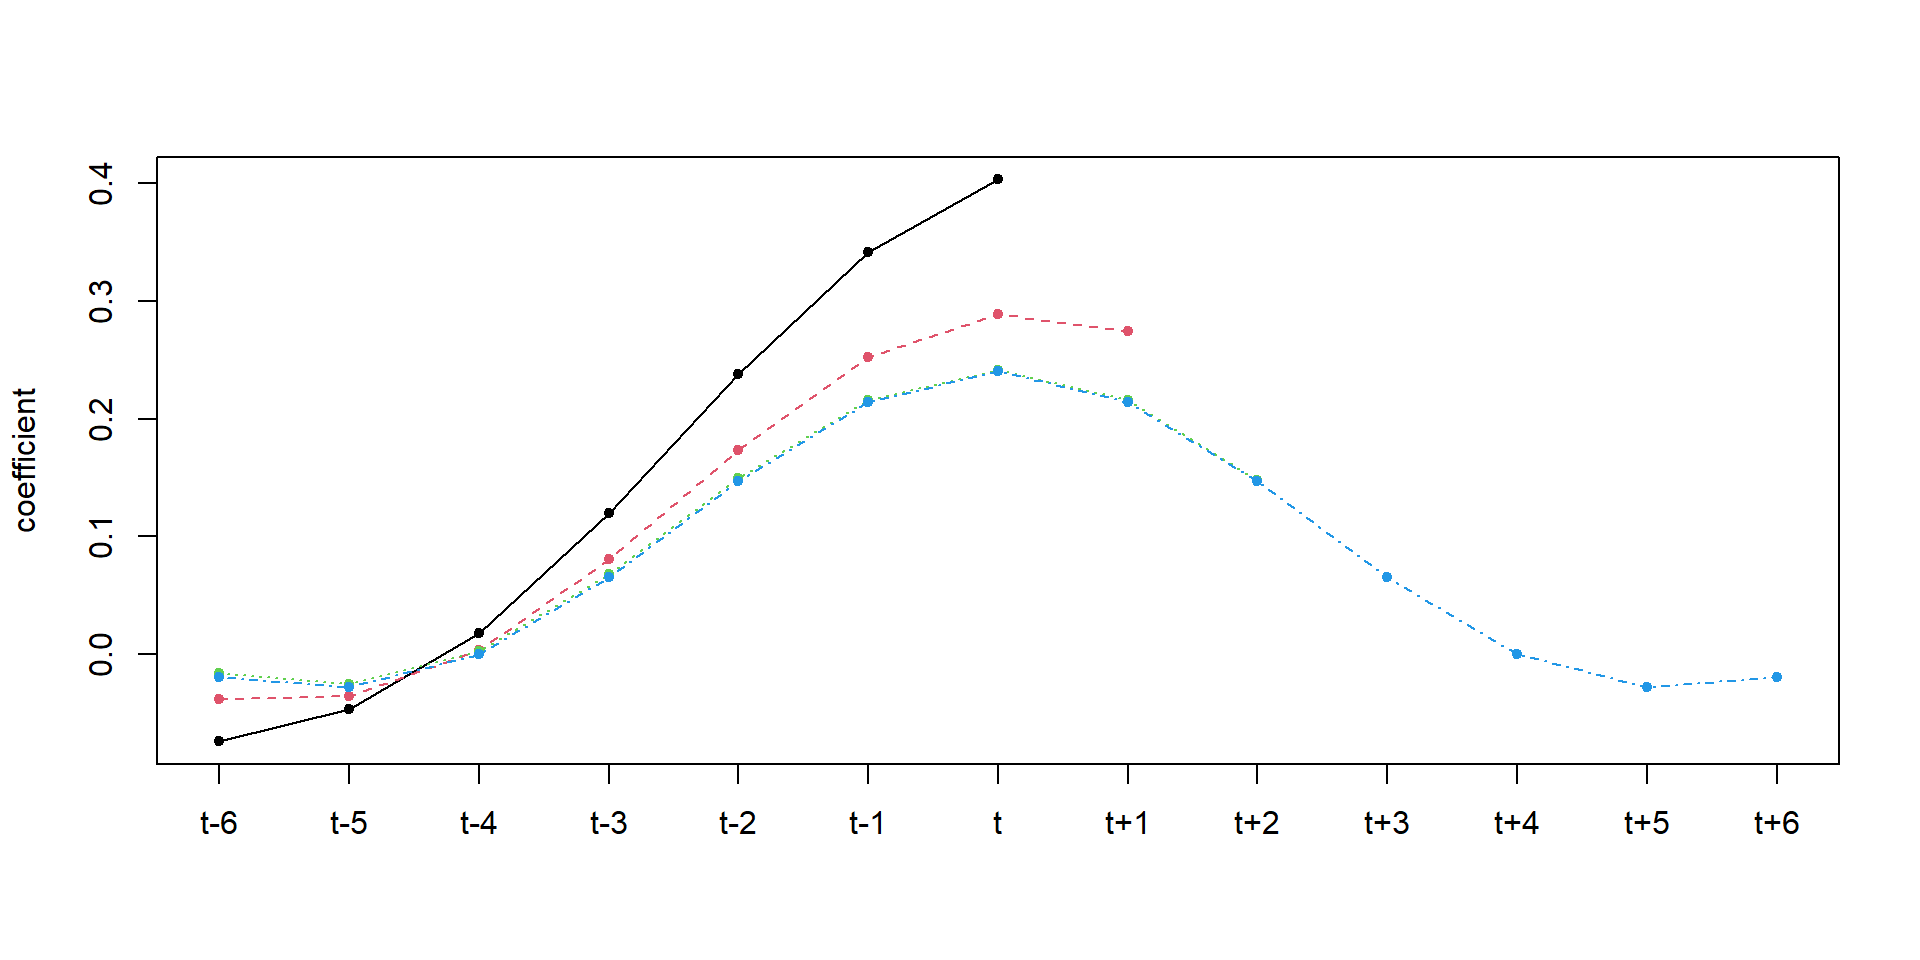
\includegraphics{NTTS_files/figure-latex/unnamed-chunk-2-1.pdf}
\caption{\label{fig:sa_ipi}Result of the seasonal adjustment process
for the french IPI in manufacturing}
\end{figure}

More complex figures are also implemented to get more details on the
components of the series, like S-I-ratio (figures
\ref{fig:sa_si_ratio}).

\begin{Shaded}
\begin{Highlighting}[]
\KeywordTok{plot}\NormalTok{(x13_ipi}\OperatorTok{$}\NormalTok{decomposition, }\DataTypeTok{ask =} \OtherTok{FALSE}\NormalTok{)}
\end{Highlighting}
\end{Shaded}%$

\begin{figure}[H]
\centering
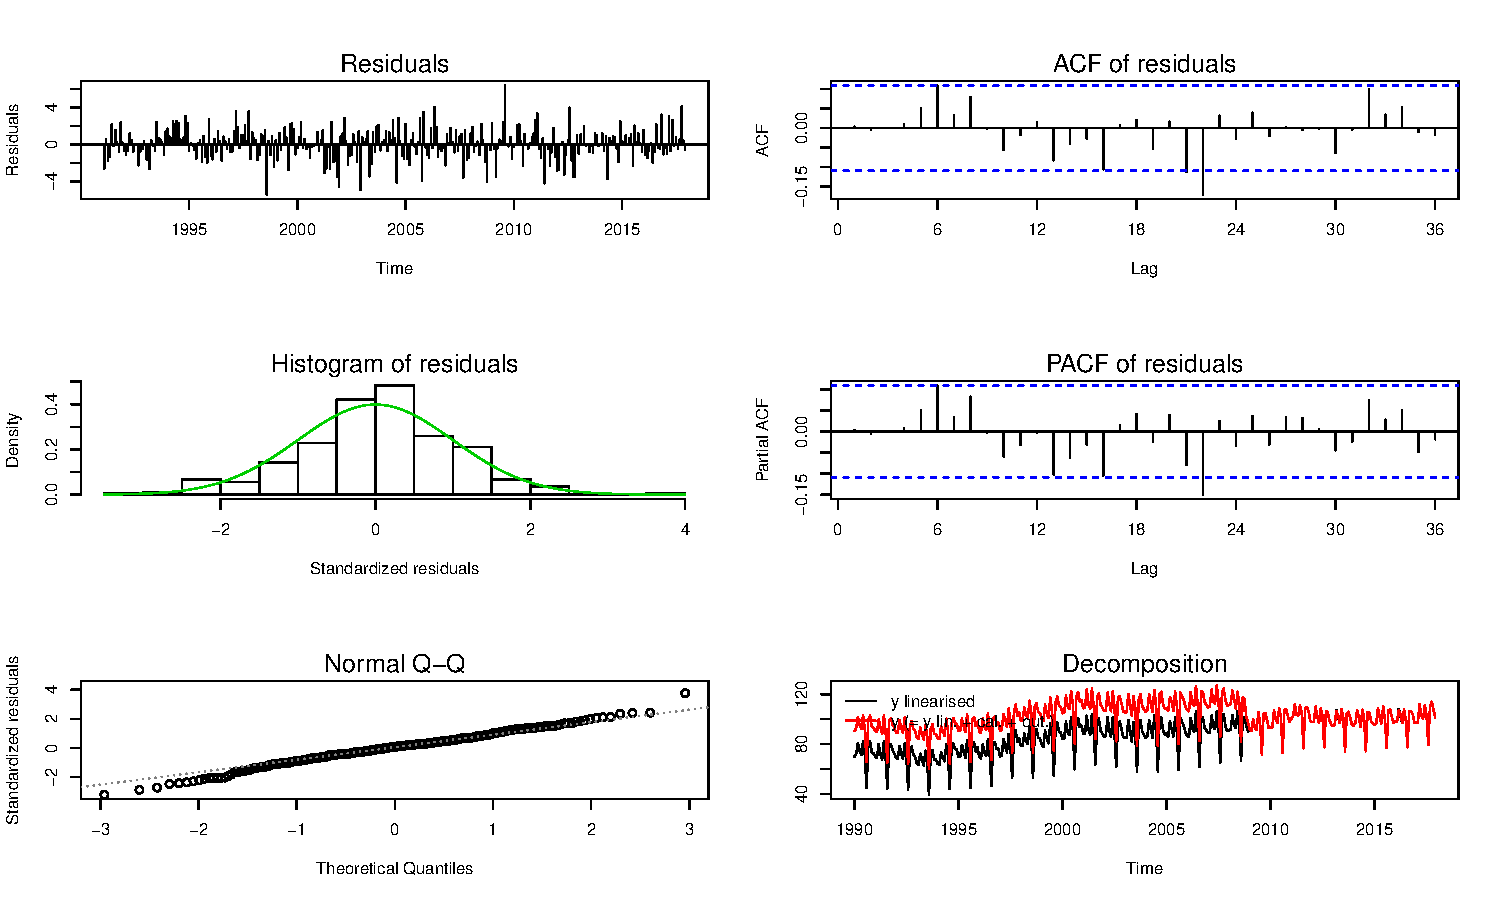
\includegraphics{NTTS_files/figure-latex/unnamed-chunk-3-1.pdf}
\caption{\label{fig:sa_si_ratio}S-I ratio}
\end{figure}

Other R libraries can also be used on the result of the seasonal
adjustment model, not available in JDemetra+. So, for example, the
Diebold-Mariano test \cite{dmtest} (implemented in the
\href{ttps://CRAN.R-project.org/package=forecast}{forecast} package) can
be used to compare the forecast accuracy of two regARIMA models, as the
Shapiro-Wilk test of normality \cite{shapiro} on the residuals of a regARIMA model:

\begin{Shaded}
\begin{Highlighting}[]
\KeywordTok{shapiro.test}\NormalTok{(x13_ipi}\OperatorTok{$}\NormalTok{regarima}\OperatorTok{$}\NormalTok{residuals)}
\end{Highlighting}
\end{Shaded}

\begin{verbatim}
## 
##  Shapiro-Wilk normality test
## 
## data:  x13_ipi$regarima$residuals
## W = 0.99401, p-value = 0.5564
\end{verbatim}

\section{Conclusions}\label{conclusions}

More user-friendly than Java libraries for non-programmers, the RJDemetra package offers many new possibilities to the users, whether to facilitate production or to carry out studies. The paper would present the main functions and the structure of the package. 

\bibliographystyle{unsrtnat}
\renewcommand{\refname}{References}
\addcontentsline{toc}{section}{References}

%%\printbibliography % when using biblatex

\bibliography{\thisfile.bib}


%\printbibliography % when using biblatex


\end{document}